\def\year{2017}\relax
%File: formatting-instruction.tex
\documentclass[letterpaper]{article} %DO NOT CHANGE THIS
\usepackage{aaai19}  %Required
\usepackage{times}  %Required
\usepackage{helvet}  %Required
\usepackage{courier}  %Required
\usepackage{url}  %Required
\usepackage{graphicx}  %Required
\frenchspacing  %Required
\setlength{\pdfpagewidth}{8.5in}  %Required
\setlength{\pdfpageheight}{11in}  %Required
%PDF Info Is Required:
  \pdfinfo{}
\setcounter{secnumdepth}{0}

\usepackage{amsmath}
\usepackage{amssymb}
\usepackage{amsthm}
\usepackage{multirow}
\usepackage{tikz}
\usetikzlibrary{arrows,automata}
\usepackage{comment}

\usepackage{graphicx}
\usepackage{caption}
\usepackage{subcaption}
\usepackage{listings}

\lstset{
  basicstyle=\ttfamily,
  mathescape
}


\usepackage{multicol}
\usepackage{arydshln}
\usetikzlibrary{calc,backgrounds,positioning,fit}


\newcommand{\tup}[1]{{\langle #1 \rangle}}

\newcommand{\pre}{\mathsf{pre}}     % precondition
\newcommand{\del}{\mathsf{del}}     % effect
\newcommand{\add}{\mathsf{add}}     % effect
\newcommand{\eff}{\mathsf{eff}}     % effect
\newcommand{\cond}{\mathsf{cond}}   % conditional effect
\newcommand{\true}{\mathsf{true}}   % true
\newcommand{\false}{\mathsf{false}} % false
\newcommand{\PE}{\mathrm{PE}}     % precondition
\newcommand{\strips}{\textsc{Strips}}     % precondition


\newtheorem{theorem}{Theorem}
\newtheorem{lemma}[theorem]{Lemma}
\newtheorem{definition}[theorem]{Definition}


\begin{document}

\title{Model Recognition as Planning}

% Commented for blind submission
\author{Diego Aineto\and Sergio Jim\'enez\and Eva Onaindia \and Miquel Ram\'irez\\
{\small Departamento de Sistemas Inform\'aticos y Computaci\'on}\\
{\small Universitat Polit\`ecnica de Val\`encia.}\\
{\small Camino de Vera s/n. 46022 Valencia, Spain}\\
{\small \{dieaigar,serjice,onaindia\}@dsic.upv.es}}



\maketitle
\begin{abstract} 
Given the partial observation of a plan execution and a set of possible planning models (models that share the same state variables but that update these variables according to different action models), {\em model recognition} is the task of identifying which model in the set explains/produced the given observation. The paper formalizes the {\em model recognition} task and introduces a novel method to estimate the probability of a \strips\ model to produce an observation of a plan execution. This method, that we called {\em model recognition as planning}, is built on top of off-the-shelf classical planning algorithms and is robust to missing intermediate states and actions in the observed plan execution. The effectiveness of {\em model recognition as planning} is shown in a set of \strips\ models encoding different kinds of {\em automata}. We show that {\em model recognition as planning} succeeds to identify the executed automata despite the internal machine state or actual applied transitions, are unobserved.
\end{abstract}

\section{Introduction}
\label{sec:introduction}
{\em Plan recognition} is the task of predicting the future actions of an agent provided observations of its current behavior~\cite{carberry2001techniques}. {\em Goal recognition} is a closely related task that aims identifying the goals of the observed agent. Goal recognition is considered {\em automated planning} in reverse; while automated planning compute sequences of actions that accounts for a given goals, goal recognition compute goals that account for an observed sequence of actions~\cite{geffner:book:2013}.

Diverse approaches has been proposed for plan/goal recognition such as {\em rule-based systems}, {\em parsing}, {\em graph-covering}, {\em Bayesian nets}, etc~\cite{sukthankar2014plan}. {\em Plan recognition as planning} is the model-based approach for plan/goal recognition~\cite{ramirez2012plan,ramirez2009plan}. This approach assumes that the action model of the observed agent is known and leverages it to compute the most likely goal of the agent, according to the observed plan execution.

This paper formalizes the {\em model recognition} task where the object to recognize is not a goal but the {\em planning model} that determines the behavior of the observed agent. Given a partial observation of a plan execution and a set of possible planning models (models that share the same state variables but that update these variables with different action models), {\em model recognition} is the task of identifying the model in the set with the highest probability of producing/explaining the given observation.

\begin{figure}
  \begin{scriptsize}    
  \begin{center}
  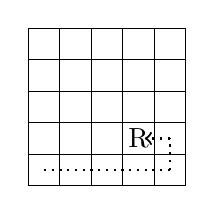
\begin{tikzpicture}[scale=.4]
          \begin{scope}
            \draw (0, 0) grid (5, 5);
            \node[anchor=center] at (3.5, 1.5) {R};
            \node[anchor=center] at (0.5, 0.5) {};
            \draw[thick,style=dotted] (0.5,0.5) -- (4.5,0.5);
            \draw[thick,style=dotted] (4.5,0.5) -- (4.5,1.5);
            \draw[thick,style=dotted,->] (4.5,1.5) -- (3.7,1.5);                        
          \end{scope}
        \end{tikzpicture}
\hspace*{1cm}        
	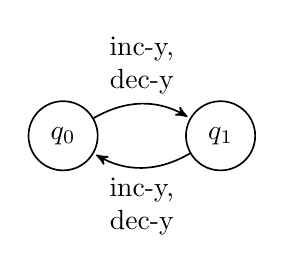
\begin{tikzpicture}[->,>=stealth',shorten >=1pt,auto,node distance=2cm,semithick]
	  \node[state] (A)              {$q_0$};
	  \node[state] (B) [right of=A] {$q_1$};          
	  \path
(A) edge [bend left, align=center] node {inc-y,\\dec-y} (B)
(B) edge [bend left, align=center] node {inc-y,\\dec-y} (A);
	\end{tikzpicture}
  \end{center}
  \end{scriptsize}  
 \caption{\small ({\em Left)} Robot navigating a $5\times 5$ grid. {\em (Right)} Automata controling that the robot only increments its x-coordinate at {\em even} rows (when $q_0$ holds, given that actions {\tt inc-y} and {\tt dec-y} update the robot y-coordinate and the automata state).}
\label{fig:grid-example}
\end{figure}

To better illustrate {\em model recognition}, imagine a robot in a $n\times n$ grid whose navigation is determined by the \strips\ model of Figure~\ref{fig:model-example}. According to this model the robot could increment its {\em x-coordinate} at {\em even rows} (when {\tt\small $q0$} holds) and decrement it at the {\em odd rows} (when {\tt\small $q1$} holds). Apart from this particular navigation model, different action models could be defined within the same state variables (e.g. altering the way {\tt\small $q0$} and {\tt\small $q1$} are required and updated) and these models can determine different kinds of robot navigation. Given an observation of a plan execution (like the one illustrated at Figure~\ref{fig:grid-example}) {\em model recognition} would aim here to identify which navigation model produced/explains that observation, despite key information is unobserved (e.g. the particular applied actions or the value of the state variables {\small\tt $q0$} and {\small\tt $q1$}). 

{\em Model recognition} is of interest because once the planning model is recognized, then the model-based machinery for automated planning becomes applicable~\cite{ghallab2004automated}. In addition, it enables identifying different kinds of automata by observing their execution. It is well-known that diverse automatae representations, like {\em finite state controllers}, {\em push-down automata}, {\em {\sc GOLOG} programs} or {\em reactive policies}, can be encoded as classical planning models~\cite{baier2007exploiting,Geffner:FSM:AAAI10,ivankovic2015optimal,segovia2017generating}.

The paper also introduces {\em model recognition as planning}; a novel method to estimate the probability of a given \strips\ model to produce an observed plan execution. Our method is built on top of off-the-shelf classical planning algorithms and is robust to missing intermediate states and actions in the observed plan execution. 

We evaluate the effectiveness of {\em model recognition as planning} with sets of \strips\ models that represent different {\em automata}. All the {\em automata} in a set are defined within the same state variables (same input {\em alphabet} and same {\em machine states}) but different {\em transition functions}. We show that {\em model recognition as planning} succeeds to identify the executed {\em automata} despite internal machine states or actual applied transitions are unobserved.

\begin{figure}
  \begin{tiny}
  \begin{verbatim}
  (:action inc-x
    :parameters (?v1 ?v2)
    :precondition (and (xcoord ?v1) (next ?v1 ?v2) (q0))
    :effect (and (not (xcoord ?v1)) (xcoord ?v2)))

  (:action dec-x
    :parameters (?v1 ?v2)
    :precondition (and (xcoord ?v1) (next ?v2 ?v1) (q1))
    :effect (and (not (xcoord ?v1)) (xcoord ?v2)))

  (:action inc-y-even
    :parameters (?y1 ?y2)
    :precondition (and (ycoord ?y1) (next ?y1 ?y2) (q0))
    :effect (and (not (ycoord ?y1)) (ycoord ?y2)
                 (not (q0)) (q1))

  (:action inc-y-odd
    :parameters (?y1 ?y2)
    :precondition (and (ycoord ?y1) (next ?y1 ?y2) (q1)))
    :effect (and (not (ycoord ?y1)) (ycoord ?y2)
                 (not (q1)) (q0)))

  (:action dec-y-even
    :parameters (?y1 ?y2)
    :precondition (and (ycoord ?y1) (next ?y2 ?y1) (q0))
    :effect (and (not (ycoord ?y1)) (ycoord ?y2)
                 (not (q0)) (q1)))

  (:action dec-y-odd
    :parameters (?y1 ?y2)
    :precondition (and (ycoord ?y1) (next ?y2 ?y1) (q1))
    :effect (and (not (ycoord ?y1)) (ycoord ?y2)
                 (not (q1)) (q0)))
  \end{verbatim}           
  \end{tiny}  
 \caption{\small Example of a \strips\ action model (codded in PDDL) for robot navigation in a $n\times n$ grid.}
\label{fig:model-example}
\end{figure}



\section{Background}
\label{sec:background}
This section formalizes the models for {\em classical planning} and for the {\em observation} of the execution of a classical plan.

\subsection{Classical planning}
We use $F$ to denote the set of {\em fluents} (propositional variables) describing a state. A {\em literal} $l$ is a valuation of a fluent $f\in F$, i.e. either~$l=f$ or $l=\neg f$. A set of literals $L$ represents a partial assignment of values to fluents (without loss of generality, we will assume that $L$ does not assign conflicting values to any fluent). We use $\mathcal{L}(F)$ to denote the set of all literal sets on $F$, i.e.~all partial assignments of values to fluents.

A {\em state} $s$ is a full assignment of values to fluents and we explicitly include negative literals $\neg f$ in states; i.e. $|s|=|F|$, so the size of the state space is $2^{|F|}$. Like in PDDL~\cite{fox2003pddl2}, we assume that fluents $F$ are instantiated from a set of {\em predicates} $\Psi$. Each predicate $p\in\Psi$ has an argument list of arity $ar(p)$. Given a set of {\em objects} $\Omega$, the set of fluents $F$ is induced by assigning objects in $\Omega$ to the arguments of predicates in $\Psi$; i.e.~$F=\{p(\omega):p\in\Psi,\omega\in\Omega^{ar(p)}\}$ such that $\Omega^k$ is the $k$-th Cartesian power of $\Omega$.

A {\em classical planning frame} is a $\tup{F,A}$ pair, where $F$ is a set of {\em fluents} and $A$ is a set of {\em actions}. The semantics of actions $a\in A$ are specified with two functions: $\rho(s,a)$ that denotes whether the action is {\em applicable} in a state $s$ and $\theta(s,a)$ that denotes the {\em successor state} that results of applying the action $a$ in a state $s$. In this work we specify action semantics (the $\rho$ and $\theta$ functions) with the \strips\ model. With this regard, an action $a\in A$ is defined by:
\begin{itemize}
\item $\pre(a)\in\mathcal{L}(F)$, the {\em preconditions} of $a$, is the set of literals that must hold for the action $a\in A$ to be applicable.
\item $\eff^+(a)\in\mathcal{L}(F)$, the {\em positive effects} of $a$, is the set of literals that are true after the application of action $a\in A$.
\item $\eff^-(a)\in\mathcal{L}(F)$, the {\em negative effects} of $a$, is the set of literals that are false after the application of the action.
\end{itemize}
We say that an action $a\in A$ is {\em applicable} in a state $s$ iff $\pre(a)\subseteq s$. The result of applying $a$ in $s$ is the {\em successor state} denoted by $\theta(s,a)=\{s\setminus\eff^-(a))\cup\eff^+(a)\}$.

A {\em classical planning problem} is a tuple $P=\tup{F,A,I,G}$, where $I$ is an initial state and $G\in\mathcal{L}(F)$ is a goal condition. A {\em plan} $\pi$ for $P$ is an action sequence $\pi=\tup{a_1, \ldots, a_n}$ that induces the {\em trajectory} $\tau(\pi,s_0)=\tup{a_1, s_1, \ldots, a_n, s_n}$ such that $s_0=I$ and, for each {\small $1\leq i\leq n$}, $a_i$ is applicable in $s_{i-1}$ and generates the successor state $s_i=\theta(s_{i-1},a_i)$. The {\em plan length} is denoted with $|\pi|=n$. A plan $\pi$ {\em solves} $P$ iff $G\subseteq s_n$, i.e.,~if the goal condition is satisfied at the last state reached after following the application of the plan $\pi$ in the initial state $I$. A solution plan for $P$ is {\em optimal} if it has minimum length.

\subsection{Conditional effects}
{\em Conditional effects} allow planning actions to have different semantics according to the value of the current state. This feature is useful for compactly defining our method for {\em model recognition as planning}. 

An action $a\in A$ with conditional effects is defined as a set of {\em preconditions} $\pre(a)\in\mathcal{L}(F)$ and a set of {\em conditional effects} $\cond(a)$. Each conditional effect $C\rhd E\in\cond(a)$ is composed of two sets of literals $C\in\mathcal{L}(F)$, the {\em condition}, and $E\in\mathcal{L}(F)$, the {\em effect}.

An action $a\in A$ is {\em applicable} in a state $s$ iff $\pre(a)\subseteq s$, and the {\em triggered effects} resulting from the action application are the effects whose conditions hold in $s$:
\[
triggered(s,a)=\bigcup_{C\rhd E\in\cond(a),C\subseteq s} E,
\]

The result of applying action $a$ in state $s$ is the {\em successor} state $\theta(s,a)=\{s\setminus\eff_c^-(s,a))\cup\eff_c^+(s,a)\}$ where $\eff_c^-(s,a)\subseteq triggered(s,a)$ and $\eff_c^+(s,a)\subseteq triggered(s,a)$ are, respectively, the triggered {\em negative} and {\em positive} effects.

\subsection{The observation model}
Given a classical planning problem $P=\tup{F,A,I,G}$ and a plan $\pi$ that solves $P$; the observation of the execution of $\pi$ on $P$ is $\mathcal{O}(\pi,I)=\tup{a_1^o,s_1^o \ldots , a_l^o, s_m^o}$, an interleaved combination of {\small $1\leq l\leq |\pi|$} observed actions and {\small $1\leq m\leq |\pi|$} observed states such that:
\begin{itemize}
\item Observed actions are {\em consistent} with $\pi$~\cite{ramirez2009plan}. This means that $\tup{a_1^o, \ldots, a_l^o}$ is a sub-sequence of the solution plan $\pi$.
\item Observed states are a sub-sequence  of partial states {\em consistent} with the sequence of states $\tup{s_0, s_1, \ldots, s_n}$ traversed by $\pi$. 
\end{itemize}

On the one hand, the initial state $I$ is fully observed while the observed states in $\mathcal{O}(\pi,I)$ may be partial, i.e. the value of certain fluents in the intermediate states may be omitted (~$|s_i^o|\leq |F|$ for every $1\leq i\leq m$). On the other hand, the sequence of observed states $\tup{s_1^o, \ldots, s_m^o}$ in $\mathcal{O}(\pi,I)$ is the same sequence of states traversed by $\pi$ but certain states may also be omitted. Formally, $0\leq|s_i^o|$ for every $1\leq i\leq m$. This means that the transitions between two consecutive observed states in $\mathcal{O}(\pi,I)$ may require the execution of more than a single action ($\theta(s_i^o,\tup{a_1,\ldots,a_k})=s_{i+1}^o$, where ${\small k\geq 1}$ is unknown and unbound). Therefore we can conclude that having $\mathcal{O}(\pi,I)$ does not implies knowing the actual length of $\pi$.

\begin{definition}[$\Phi$-observation]
Given a subset of fluents $\Phi\subseteq F$ we say that $\mathcal{O}(\pi,I)$ is a $\Phi$-observation of the execution of $\pi$ on $P$ iff, for every ${\small 1\leq i\leq m}$, each observed state $s_i^o$ only contains fluents in $\Phi$.
\end{definition}

Figure~\ref{fig:grid-example} illustrates the six-state $\Phi$-observation \{{\tt\footnotesize<(xcoord 2)(ycoord 1)>, <(xcoord 3)(ycoord 1)>, <(xcoord 4)(ycoord 1)>, <(xcoord 5)(ycoord 1)>, <(xcoord 5)(ycoord 2)>, <(xcoord 4)(ycoord 2)>}\}, where $\Phi$ only contains fluents of the kind {\tt\small (xcoord ?v)} and {\tt\small (ycoord ?v)}. This means that, for each observed state, only the value of fluents {\tt\small (xcoord ?v)} and {\tt\small (ycoord ?v)} is known while the value of the remaining fluents, namely {\tt\small (next ?v1 ?v2)}, {\tt\small (q0)} and {\tt\small (q1)}, is unknown.



\section{Model Recognition}
\label{sec:recognition}
The {\em model recognition} task is a tuple $\tup{P,M,\mathcal{O}}$ where:
\begin{itemize}
\item $P=\tup{F,A[\cdot],I,G}$ is a {\em classical planning problem} s.t. the semantics of actions $a\in A[\cdot]$ is unknown, i.e. the corresponding functions $\rho(s,a)$ and/or $\theta(s,a)$ are undefined.
\item $M=\{\mathcal{M}_1,\ldots,\mathcal{M}_m\}$ is a finite non-empty {\em set of models} for the actions in $A$ s.t., each model in $\mathcal{M}\in M$, defines different function pairs $\tup{\rho,\theta}$ over the state variables $F$.
\item $\mathcal{O}(\pi,I)$ is an {\em observation} of the execution of an unknown solution plan $\pi$ for the planning problem $P$.
\end{itemize}

{\em Model recognition} can be understood as a {\em classification task} where each class is represented with a different planning model $\mathcal{M}\in M$ and the observed plan execution $\mathcal{O}(\pi,I)$ is the single example to classify. Further, the planning model associated to each class acts as the corresponding {\em class prototype} that summarizes all the plan executions that could be synthesized with that model (i.e. all the examples that belong to that class).

In this work we follow the {\em naive Bayes classifier} to assign a model $\mathcal{M}\in M$ to the given observation $\mathcal{O}(\pi,I)$ with respect to the expression:
\begin{align}
argmax_{\mathcal{M}\in M} P(\mathcal{O}|\mathcal{M})\times P(\mathcal{M}).
\end{align}
The hypotheses in {\em model recognition} are then about the possible action models $\mathcal{M}\in M$, while the observation $\mathcal{O}(\pi,I)$ of a plan execution represents the input observation. The {\em solution} to the {\em model recognition} task is the model $\mathcal{M}\in M$ (or subset of models in $M$) that maximizes the previous expression.

The $P(\mathcal{M})$ probability expresses whether one model is known to be a priori more likely than the others. If this probability is not given as input it is reasonable to assume that {\em a priori} all models are equiprobable. The challenge in our formulation for {\em model recognition} is the definition of the $P(\mathcal{O}|\mathcal{M})$ {\em likelihood} that expresses the probability of observing $\mathcal{O}(\pi,I)$ when $\mathcal{M}$ is the planning model.

\begin{figure}
  \begin{scriptsize}
  \begin{center}
	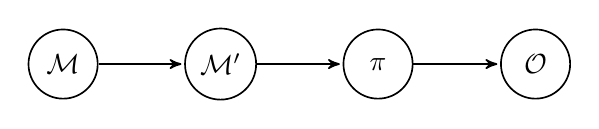
\begin{tikzpicture}[->,>=stealth',shorten >=1pt,auto,node distance=2cm,semithick]
	  \node[state] (A)              {$\mathcal{M}$};
	  \node[state] (B) [right of=A] {$\mathcal{M}'$};
	  \node[state] (C) [right of=B] {$\pi$};
	  \node[state] (D) [right of=C] {$\mathcal{O}$};          
	  \path
(A) edge  node {} (B)
(B) edge  node {} (C)
(C) edge  node {} (D)
;
	\end{tikzpicture}
  \end{center}
  \end{scriptsize}  
 \caption{\small {\em Bayesian network} abstracting that model $\mathcal{M}'$ results from editing $\mathcal{M}$ and that can produce a plan $\pi$ consistent with $\mathcal{O}(\pi,I)$.}
\label{fig:net}
\end{figure}

Our approach to formulate the $P(\mathcal{O}|\mathcal{M})$ {\em likelihood} is to assess how far is $\mathcal{M}$ from a model $\mathcal{M'}$ that can produce a plan $\pi$ that solves $P$ and s.t. $\mathcal{O}(\pi,I)$ is a {\em consistent} observation of the execution of $\pi$ on $P$. Figure~\ref{fig:net} shows the four-variable {\em Bayesian network} abstracting this process. Regarding this network we have that:
\begin{align}
 P(\mathcal{O}|\mathcal{M})=\sum_{\mathcal{M}'}\sum_{\pi} P(\mathcal{M'}|\mathcal{M})P(\pi|\mathcal{M'})P(\mathcal{O}|\pi),
\end{align}
where $\mathcal{M}'$ ranges over all the models that can be generated editing $\mathcal{M}$ and $\pi$ ranges over all the plans that can be synthesized with a model $\mathcal{M}'$

\subsection{Approximating the $P(\mathcal{O}|\mathcal{M})$ {\em likelihood}}
Following the previous equation (2) the exact computation of $P(\mathcal{O}|\mathcal{M})$ is intractable because, for most planning problems, the set of {\em valid} plans consistent with an observation can easily be very large (infinite in the case of planning problems without dead-ends). Instead, in this work we propose to estimate $P(\mathcal{O}|\mathcal{M})$ making the following assumptions:
\begin{enumerate}
\item The sum in the previous equation is dominated by the {\em closest compliant set}, i.e. the models closest to $\mathcal{M}$ that can produce a solution plan consistent with $\mathcal{O}(\pi,I)$. The rationale behind this assumption is that the further the compliant model, the lower the $P(\mathcal{O}|\mathcal{M})$ likelihood. 
\end{enumerate}

The {\em full observability of the executed plan} is a too strong assumption but, as we explain next, it allows us to build reasonable estimates of the $P(\mathcal{O}|\mathcal{M})$ {\em likelihood} for the more general case where the observability of the executed plan is partial.

Note that in this baseline scenario where there is {\em full observability of the executed plan}:
\begin{itemize}
\item There is only a single possible plan {\em consistent} with the given observation, besides $P(\mathcal{O}|\pi)=1$.
\item If we consider assumption 1, the {\em closest compliant set} $\mathcal{M}^*$ becomes a singleton for this particular scenario, so that probabilities corresponding to different compliant models are not added up. Further, the $P(\pi|\mathcal{M^*})$ probability equals also to $1$ since there is only one possible plan consistent with the observation and by definition, the {\em closest compliant} model produces that plan.
\end{itemize}
As a consequence, when there is {\em full obsevability of the executed plan} and under the previous assumption, we have that expression (1) simplifies to
\begin{align}
argmax_{\mathcal{M}\in M} P(\mathcal{M^*}|\mathcal{M}).
\end{align}

Next we show how to approximate the $P(\mathcal{O}|\mathcal{M})$ {\em likelihood} for the more general case where there is partial observability of the executed plan. First we start with the simpler scenario where the length of the observed plan is bound and add these two new assumptions.
\begin{enumerate}\addtocounter{enumi}{1}
\item The {\em closest compliant set} is a singleton, so that probabilities corresponding to different compliant models are not added up.
\item All solutions of a given {\em plan length} are equiprobable, with shorter plans more likely than longer plans.  
\end{enumerate}

In such an scenario $P(\mathcal{O}|\pi)$ equals to a constant $\alpha$ that indicates the number of plans of bounded length that are consistent with $\mathcal{O}$. Likewise, $P(\pi|\mathcal{M^*})$ is also one given the definition of the {\em closest compliant set}. As a consequence, when there is {\em partial obsevability of the executed plan} (but the plan length is bound), and under the previous three assumptions, we have that expression (1) simplifies to
\begin{align}
argmax_{\mathcal{M}\in M} P(\mathcal{M^*}|\mathcal{M})\times \alpha.
\end{align}
where $\alpha$ is a normalizing constant that has the same value for every $\mathcal{M}\in M$, so it can be ignored.


Finally, we can say that the $P(\mathcal{O}|\mathcal{M})$ {\em likelihood} can be estimated for the general case of partial observability of the executed plan (where the length of the plan is not bound) by adding a fourth assumption:
\begin{enumerate}\addtocounter{enumi}{3}
\item The observed plan $\pi$ that solves $P$ is an optimal plan since we are assuming that the observed agent is acting rationally~\cite{ramirez2012plan}.
\end{enumerate}
In this case the length of the plan becomes bound by the optimal plan length and hence, we can again use expression (4) for the  likelihood estimation.





\section{Recognition of \strips\ models}
\label{sec:asPlanning}
Here we analyze the particular instantiation of the {\em model recognition} task where the semantics of actions (i.e. $\rho$ and $\theta$ functions) are specified with \strips\ action schemas. We start formalizing the \strips\ schema and define the full space of possible \strips\ schema. Eventually, we introduce an {\em edit distance} for \strips\ schema to estimate the $P(\mathcal{O}|\mathcal{M})$ likelihoods for classical planning models.

\subsection{Well-defined \strips\ action schema}
\strips\ action schema provide a compact representation for specifying classical planning models. For instance, Figure~\ref{fig:model-example} shows six \strips\ action schema, codded in PDDL, that determine a particular kind of robot navigation in $n\times n$ grids.

A \strips\ action schema $\xi$ is defined by a list of {\em parameters} $pars(\xi)$, and three list of predicates (namely $pre(\xi)$, $del(\xi)$ and $add(\xi)$) that shape the kind of fluents that can appear in the {\em preconditions}, {\em negative effects} and {\em positive effects} of the actions induced from that schema.

We say that two \strips\ schemes $\xi$ and $\xi'$ are {\em comparable} iff $pars(\xi)=pars(\xi')$, both share the same list of parameters. For instance, we claim that the six action schema of Figure~\ref{fig:model-example} are {\em comparable} while, for example, the {\small\tt stack(?v1,?v2)} and {\small\tt pickup(?v1)} schemes from the four opertator {\em blocksworld}~\cite{slaney2001blocks} are not. Last but not least, we say that two \strips\ models $\mathcal{M}$ and $\mathcal{M}'$ are {\em comparable} iff there exists a bijective function $\mathcal{M} \mapsto \mathcal{M}^*$ that maps every action schema $\xi\in\mathcal{M}$ to a comparable schema $\xi'\in\mathcal{M'}$ and vice versa.

Given a \strips\ action schema $\xi$, let us define an additional set of objects ($\Omega\cap\Omega_\xi=\emptyset$), that we denote as {\em variable names}, and that contains one variable name for each parameter in $pars(\xi)$, that is $\Omega_\xi=\{v_i\}_{i=1}^{|pars(\xi)|}$. For any of the six schema defined in Figure~\ref{fig:model-example}, $|pars(\xi)|=2$ so $\Omega_\xi=\{v_1,v_2\}$.

Given a \strips\ action schema $\xi$ and a set of {\em predicates} $\Psi$ that shape the propositional state variables. The set of FOL interpretations of $\Psi$ over the corresponding $\Omega_\xi$ objects (the {\em variable names} for schema $\xi$), confines the elements that can appear in the $pre(\xi)$, $del(\xi)$ and $add(\xi)$ lists. We denote this set of FOL interpretations as ${\mathcal I}_{\Psi,\xi}$. For any of the six schema defined in Figure~\ref{fig:model-example} the ${\mathcal I}_{\Psi,\xi}$ set contains the same ten elements, ${\mathcal I}_{\Psi,\xi}=${\small\tt\{xcoord($v_1$), xcoord($v_2$), ycoord($v_1$), ycoord($v_2$), q0(), q1(), next($v_1$,$v_1$), next($v_1$,$v_2$), next($v_2$,$v_1$), next($v_2$,$v_2$))\}}.

Despite any element from ${\mathcal I}_{\Psi,\xi}$ can {\em a priori} appear in the $pre(\xi)$, $del(\xi)$ and $add(\xi)$ lists of a schema $\xi$. The space of possible \strips\ schema is bound further by ${\mathcal C}$, a set of constraints of the following kinds: 
\begin{itemize}
\item {\em Syntactic constraints}. \strips\ constraints require negative effects appearing as preconditions, negative effects cannot be positive effects at the same time and also, positive effects cannot appear as preconditions. Formally, $del(\xi)\subseteq pre(\xi)$, $del(\xi)\cap add(\xi)=\emptyset$ and $pre(\xi)\cap add(\xi)=\emptyset$). Considering exclusively these syntactic constraints, the size of the space of possible \strips\ schema is given by the expression, $2^{2\times|{\mathcal I}_{\Psi,\xi}|}$. For the navigation model of Figure~\ref{fig:model-example}, $2^{2\times 10}=1,048,576$ for every action schema.
\item {\em Domain-specific constraints}. One can also introduce domain-specific knowledge to more precisely bound the space of possible \strips\ schema for a particular domain. For instance, in a {\em robot navigation} model, like the one in Figure~\ref{fig:model-example}, {\small\tt q0()} and {\small\tt q1()} are exclusive so they cannot hold a the same time in a $pre(\xi)$/$del(\xi)$/$add(\xi)$ list. Further, {\small\tt next($v_1$,$v_1$)} and {\small\tt next($v_2$,$v_2$)} will not appear at any of these lists because the {\tt\small next} predicate is coding the {\em succesor} function for {\em natural numbers}. In this case, introducing these domain-specific constraints reduces the size of the space of possible schema to $2^{2\times 7}=16,384$ for every action schema.
\end{itemize}

Now we are ready to define what is a {\em well-defined} \strips\ action schema.
\begin{definition}[Well-defined \strips\ action schema]
Given a set of {\em predicates} $\Psi$, a list of action {\em parameters} $pars(\xi)$, and set of FOL constraints ${\mathcal C}$ we say that $\xi$ is a {\bf well-defined \strips\ action schema} iff its three lists $pre(\xi)\subseteq {\mathcal I}_{\Psi,\xi}$, $del(\xi)\subseteq{\mathcal I}_{\Psi,\xi}$ and $add(\xi)\subseteq{\mathcal I}_{\Psi,\xi}$ only contain elements in ${\mathcal I}_{\Psi,\xi}$ and they satisfy all the constraints in ${\mathcal C}$. 
\end{definition}
We say that an action model is {\em well-defined} if all its \strips\ action schema are {\em well-defined}.

\subsection{Edit distances for \strips\ action models}
{\em Edit distances} are similarity metrics, traditionally computed over {\em strings} or {\em graphs}, and that has been proved successful for {\em pattern recognition}~\cite{masek1980faster,bunke1997relation}. In this work we formalize and compute edit distances that are referred to \strips\ planning models.  First, we define two edit \emph{operations} on a schema $\xi\in\mathcal{M}$ that belongs to a \strips\ action model $\mathcal{M}\in M$:
\begin{itemize}
\item {\em Deletion}. An element is removed from any of these three lists $pre(\xi)$, $del(\xi)$ and $add(\xi)$ of the operator schema $\xi\in\mathcal{M}$ such that the resulting schema is a {\em well-defined} \strips\ action schema.
\item {\em Insertion}. An element in ${\mathcal I}_{\Psi,\xi}$ is added to any of these three lists $pre(\xi)$, $del(\xi)$ and $add(\xi)$ of the operator schema $\xi\in\mathcal{M}$ s.t. the resulting schema is {\em well-defined}.
\end{itemize}

We can now formalize an {\em edit distance} that quantifies how similar two given \strips\ action models are. The distance is symmetric and meets the {\em metric axioms} provided that the two {\em edit operations}, deletion and insertion, have the same positive cost.

\begin{definition}[Edit distance]
  Let $\mathcal{M}$ and $\mathcal{M}'$ be two {\em comparable} and {\em well-defined} \strips\ action models defined within the same set of predicates $\Psi$. The {\bf edit distance} $\delta(\mathcal{M},\mathcal{M}')$ is the minimum number of {\em edit operations} that is required to transform $\mathcal{M}$ into $\mathcal{M}'$.
\end{definition}

Since ${\mathcal I}_{\Psi,\xi}$ are bound sets, the maximum number of edits that can be introduced to a given action model is bound as well. 
\begin{definition}[Maximum edit distance]
The \textbf{maximum edit distance} of an \strips\ model $\mathcal{M}$ built within the set of predicates $\Psi$ is $\delta(\mathcal{M},*)=\sum_{\xi\in\mathcal{M}} 3\times|{\mathcal I}_{\Psi,\xi}|$.
\end{definition}

The observation of a plan execution, generated with an action model $\mathcal{M}$, reflects {\em semantic knowledge} that constrain further the space of the possible schema $\xi\in \mathcal{M}$. In this case, we talk about {\em observation constraints} (that can also be included into the $\mathcal{C}$ set). In addition, {\em observation constraints} allow us to define an edit distance to asses the matching of a \strips\ model with respect to an observation of a plan execution. 

\begin{definition}[Observation edit distance]
  Given $\mathcal{O}(\pi,I)$, an observation of the execution of a plan for solving $P$ and a \strips\ action model $\mathcal{M}$, all defined within the same set of predicates $\Psi$. The {\bf observation edit distance}, $\delta(\mathcal{M},\mathcal{O})$, is the minimal edit distance from $\mathcal{M}$ to any {\em comparable} and well-defined model $\mathcal{M}'$ s.t. $\mathcal{M}'$ produces a plan $\pi$ that solves $P$ and that is {\em consistent} with $\mathcal{O}(\pi,I)$; \[\delta(\mathcal{M},\mathcal{O})=\min_{\forall \mathcal{M}' \rightarrow \mathcal{O}} \delta(\mathcal{M},\mathcal{M}')\]
\end{definition}

Remarkably, the {\em observation edit distance} allows us to elicit the likelihood of the observations given a candidate model. It can be argued that the shorter this  distance the better the given model explains the given observation. Note that the {\em observation edit distance} could also be defined assessing the edition required by the observed plan execution to match the given model. This implies defining {\em edit operations} that modify the observation $\mathcal{O}(\pi,I)$ instead of $\mathcal{M}$~\cite{sohrabi:precognition:IJCAI2016}. Our definition of the {\em observation edit distance} is more practical since normally ${\mathcal I}_{\Psi,\xi}$ is much smaller than $F$. In practice, the number of {\em variable objects} should be smaller than the number of objects in a planning problem.

\begin{definition}[{\em Closest compliant models}] \label{compliant}
Given a model $\mathcal{M}$. The {\bf closest compliant models}, $\mathcal{M^*}$, is the comparable set of action models closest to $\mathcal{M}$ (in terms of editions) that can produce a solution plan consistent with $\mathcal{O}(\pi,I)$;
  \[\mathcal{M^*}=\underset{\forall \mathcal{M}' \rightarrow \mathcal{O}}{\arg\min}\ \delta(\mathcal{M},\mathcal{M}') \]
\end{definition}

\begin{figure}
{\tt\tiny
\begin{tabular}{ll}
00 : (insert\_pre\_xcoord\_v1\_inc-x)   & 07 : (validate\_0)\\
01 : (insert\_pre\_next\_v1\_v2\_inc-x) & 08 : (editable\_inc-x 1 2)\\
02 : (insert\_pre\_q0\_inc-x)           & 09 : (editable\_inc-x 2 3)\\
03 : (delete\_del\_xcoord\_v2\_inc-x)   & 10 : (editable\_inc-x 3 4) \\
04 : (delete\_add\_xcoord\_v1\_inc-x)   & 11 : (editable\_inc-x 4 5)\\
05 : (insert\_del\_xcoord\_v1\_inc-x)   & 12 : (editable\_inc-y-even 1 2)\\
06 : (insert\_add\_xcoord\_v2\_inc-x)   & 13 : (editable\_dec-x 5 4)\\
& 14 : (validate\_1)
\end{tabular}
}
 \caption{\small Plan for editing (steps [0-6]) and validating (steps [7-14]) the planning model of Figure\ref{fig:model-example} when action {\tt\small inc-x} has no preconditions and positive/negative effects are swapped wrt Figure\ref{fig:model-example}.}
\label{fig:plan-pdistance}
\end{figure}



\section{Model Recognition as classical planning}
This section shows that, for \strips\ planning models, $\delta(\mathcal{M},\mathcal{O})$ can be computed (and hence an approximation of the $P(\mathcal{O}|\mathcal{M})$ likelihood) with a compilation of a classical planning with conditional effects.

The compilation is an extension of the classical planning compilation for the learning of \strips\ planning models~\cite{aineto2018learning}. The intuition behind this compilation is that a solution to the resulting classical planning task is a sequence of actions that:
\begin{enumerate}
\item {\bf Edits the action model $\mathcal{M}$ to build $\mathcal{M}'$}. A solution plan starts with a {\em prefix} that modifies the preconditions and effects of the action schemes in $\mathcal{M}$ using to the two {\em edit operations} defined above, {\em deletion} and {\em insertion}. 
\item {\bf Validates the edited model $\mathcal{M}'$}. The solution plan continues with a postfix that:
\begin{enumerate}
\item Induces a solution plan $\pi$ for the original classical planning problem $P$.
\item Validates that $\mathcal{O}(\pi,I)$ is an observation of the execution of $\pi$ on the classical planning problem $P$.
\end{enumerate}
\end{enumerate}

Figure~\ref{fig:plan-pdistance} shows the plan with a prefix ({\em steps [0,6]}) for editing the planning model of Figure\ref{fig:model-example} when its schema {\tt\small inc-x} is defined without preconditions and its positive/negative effects are swapped wrt Figure~\ref{fig:model-example}. The postfix of the plan ({\em steps [7,14]}) validates the edited action model at the observation of the plan execution illustrated at Figure~\ref{fig:grid-example}. 

Note that our interest is not in $\mathcal{M}'$, the edited model resulting from the compilation, but in the number of required {\em edit operations} (insertions and deletions) required by $\mathcal{M}'$ to be validated. In the example of Figure~\ref{fig:plan-pdistance} $\delta(\mathcal{M},\mathcal{O})=7$ and $\delta(\mathcal{M},*)=6\times 3\times 10$ since there are 6 action schemes for which $|{\mathcal I}_{\Psi,\xi}|=10$.

\begin{figure}
\begin{tiny}
\begin{verbatim}
;;; Propositional encoding for inc-x(?v1 ?v2)
(pre_xcoord_v1_inc-x) (pre_next_v1_v2_inc-x) 
(pre_q0__inc-x)
(del_xcoord_v1_inc-x) (add_xcoord_v2_inc-x)

;;; Propositional encoding for dec-x(?v1 ?v2)
(pre_xcoord_v1_dec-x) (pre_next_v2_v1_dec-x) 
(pre_q1___dec-x)
(del_xcoord_v1_dec-x) (add_xcoord_v2_dec-x)

;;; Propositional encoding for inc-y-even(?v1 ?v2)
(pre_ycoord_v1_inc-y-even) (pre_next_v1_v2_inc-y-even)
(pre_q0__inc-y-even)
(del_ycoord_v1_inc-y-even) (del_q0__inc-y-even)
(add_ycoord_v2_inc-y-even) (add_q1__inc-y-even)

;;; Propositional encoding for inc-y-odd(?v1 ?v2)
(pre_ycoord_v1_inc-y-odd) (pre_next_v1_v2_inc-y-odd) 
(pre_q0__inc-y-odd)
(del_ycoord_v1_inc-y-odd) (del_q1__inc-y-odd)
(add_ycoord_v2_inc-y-odd) (add_q0__inc-y-odd)

;;; Propositional encoding for dec-y-even(v1 ?v2)
(pre_ycoord_v1_dec-y-even) (pre_next_v2_v1_dec-y-even)
(pre_q0__dec-y-even)
(del_ycoord_v1_dec-y-even) (del_q0__dec-y-even)
(add_ycoord_v2_dec-y-even) (add_q1__dec-y-even)

;;; Propositional encoding for dec-y-odd(?v1 ?v2)
(pre_ycoord_v1_dec-y-odd) (pre_next_v2_v1_dec-y-odd)
(pre_q1__dec-y-odd)
(del_ycoord_v1_dec-y-odd) (del_q1__dec-y-odd)
(add_ycoord_v2_dec-y-odd) (add_q0__dec-y-odd)
\end{verbatim}
\end{tiny}
 \caption{\small Propositional encoding for the six schema from Figure~\ref{fig:model-example}.}
\label{fig:encoding}
\end{figure}

\subsection{A propositional encoding for \strips\ action schema}
Given a \strips\ action schema $\xi$, a propositional encoding for the {\em preconditions}, {\em negative} and {\em positive} effects of that schema can be represented with the fluents of the kind $[pre|del|add]\_e\_\xi$ such that $e\in{\mathcal I}_{\Psi,\xi}$ is a single element from the set of interpretations of predicates $\Psi$ over the corresponding objects $\Omega_\xi$. Figure~\ref{fig:encoding} shows the propositional encoding for the six action schema defined in Figure~\ref{fig:model-example}.

The interest of having a propositional encoding for \strips\ action schema is that, using {\em conditional effects}, it allows to compactly define {\em editable actions}. Actions whose semantics is given by the value of the $[pre|del|add]\_e\_\xi$ fluents on the current state. Given an operator schema $\xi\in\mathcal{M}$ its {\em editable} version is formalized as:
\begin{small}  
\begin{align*}
\hspace*{7pt}\pre(\mathsf{editable_{\xi}})=&\{pre\_e\_\xi\implies e\}_{\forall e\in{\mathcal I}_{\Psi,\xi}}\\
\cond(\mathsf{editable_{\xi}})=&\{del\_e\_\xi\}\rhd\{\neg e\}_{\forall e\in{\mathcal I}_{\Psi,\xi}},\\
&\{add\_e\_\xi\}\}\rhd\{e\}_{\forall e\in{\mathcal I}_{\Psi,\xi}}.
\end{align*}
\end{small}

Figure~\ref{fig:editable} shows the PDDL encoding of the {\em editable version} of the {\tt\small inc-x(?v1,?v2)} schema for robot navigation in a $n\times n$ grid (see Figure~\ref{fig:model-example}). Note that this editable schema, when the fluents of Figure~\ref{fig:encoding} hold, behaves exactly as defined in Figure~\ref{fig:model-example}. 

\begin{figure}
  \begin{tiny}  
  \begin{verbatim}
(:action editable_inc-x
  :parameters (?v1 ?v2)
  :precondition
    (and (or (not (pre_xcoord_v1_inc-x)) (xcoord ?v1))
         (or (not (pre_xcoord_v2_inc-x)) (xcoord ?v2))
         (or (not (pre_ycoord_v1_inc-x)) (xcoord ?v1))                       
         (or (not (pre_ycoord_v2_inc-x)) (xcoord ?v2))
         (or (not (pre_q0__inc-x)) (q0))
         (or (not (pre_q1__inc-x)) (q1)))
         (or (not (pre_next_v1_v1_inc-x)) (next ?v1 ?v1)))
         (or (not (pre_next_v1_v2_inc-x)) (next ?v1 ?v2)))
         (or (not (pre_next_v2_v1_inc-x)) (next ?v2 ?v1)))
         (or (not (pre_next_v2_v2_inc-x)) (next ?v2 ?v2))))
    :effect (and
       (when (del_xcoord_v1_inc-x) (not (xcoord ?v1)))
       (when (del_xcoord_v2_inc-x) (not (xcoord ?v2)))
       (when (del_ycoord_v1_inc-x) (not (xcoord ?v1)))
       (when (del_ycoord_v2_inc-x) (not (xcoord ?v2)))
       (when (del_q0__inc-x) (not (q0)))
       (when (del_q1__inc-x) (not (q1)))
       (when (del_next_v1_v1_inc-x) (not (next ?v1 ?v1)))
       (when (del_next_v1_v2_inc-x) (not (next ?v1 ?v2)))
       (when (del_next_v2_v1_inc-x) (not (next ?v2 ?v1)))
       (when (del_next_v2_v2_inc-x) (not (next ?v2 ?v2)))
       
       (when (add_xcoord_v1_inc-x) (xcoord ?v1))
       (when (add_xcoord_v2_inc-x) (xcoord ?v2))
       (when (add_ycoord_v1_inc-x) (xcoord ?v1))
       (when (add_ycoord_v2_inc-x) (xcoord ?v2))
       (when (add_q0__inc-x) (q0))
       (when (add_q1__inc-x) (q1))
       (when (add_next_v1_v1_inc-x) (next ?v1 ?v1))
       (when (add_next_v1_v2_inc-x) (next ?v1 ?v2))
       (when (add_next_v2_v1_inc-x) (next ?v2 ?v1))
       (when (add_next_v2_v2_inc-x) (next ?v2 ?v2)))
  \end{verbatim}           
  \end{tiny}  
 \caption{\small Editable version of the {\tt\small inc-x(?v1,?v2)} schema for robot navigation in a $n\times n$ grid.}
\label{fig:editable}
\end{figure}


\subsection{The compilation formalization}
Conditional effects allow us to compactly define our compilation for computing $\delta(\mathcal{M},\mathcal{O})$ and hence, estimate the $P(\mathcal{O}|\mathcal{M})$ likelihood. Given a \strips\ model $\mathcal{M}\in M$ and the observation $\mathcal{O}(\pi,I)$ of the execution of a plan for solving $P=\tup{F,A,I,G}$, our compilation outputs a classical planning task with conditional effects $P'=\tup{F',A',I',G'}$ such that:
\begin{itemize}
\item $F'$ extends the original fluents $F$ with:
\begin{itemize}
\item Fluents $[pre|del|add]\_e\_\xi$ to model the possible \strips\ schema. 
\item The fluents to code the {\em observation constraints}:
\begin{itemize}
\item $F_{\pi}=\{plan(name(a_i),\Omega^{ar(a_i)},i)\}_{\small 1\leq i\leq l}$ to code the $i^{th}$ action in $\mathcal{O}(\pi,I)$. The static facts $next_{i,i+1}$ and the fluents $at_i$, {\small $1\leq i< l$}, are also added to iterate through the $l$ actions in $\mathcal{O}(\pi,I)$.
\item The fluents $\{test_j\}_{1\leq j\leq m}$, indicating the state observation $s_j\in\mathcal{O}(\pi,I)$ where the action model is validated.
\end{itemize}
\item The fluents $mode_{edit}$ and $mode_{val}$ to indicate whether the operator schemas are edited or validated.
\end{itemize}
\item $I'$ extends the original initial state $I$ with the fluent $mode_{edit}$ set to true as well as the fluents $F_{\pi}$ plus fluents $at_1$ and $\{next_{i,i+1}\}$, {\small $1\leq i<l$}, for tracking the plan step where the action model is validated. Our compilation assumes that initially $\mathcal{M}'$ is defined as $\mathcal{M}$. Therefore fluents $[pre|del|add]\_e\_\xi$ hold as given by $\mathcal{M}$.

\item $G'=G\bigcup\{at_n,test_m\}$.
\item $A'$ comprises three kinds of actions with conditional effects:
\begin{enumerate}
\item The {\em editable} version of the original actions in $A$. This actions have now an extra preconditions because they can only be applied in the {\em validation} mode (i.e. when $mode_{val}$ holds). When the observation $\mathcal{O}(\pi,I)$ includes observed actions, they also include the extra conditional effects $\{at_{i},plan(name(a_i),\Omega^{ar(a_i)},i)\}\rhd\{\neg at_{i},at_{i+1}\}_{\forall i\in [1,l]}$ to validate that actions are applied, exclusively, in the same order as they appear in $\mathcal{O}(\pi,I)$.\\

\item Actions for {\em editing} operator schema $\xi\in\mathcal{M}$. This includes the actions for {\em inserting} a new {\em precondition} into an action schema $\xi\in\mathcal{M}$ and for inserting a new {\em negative} or {\em positive} effect into the action schema $\xi\in\mathcal{M}$
\begin{small}
\begin{align*}
\hspace*{7pt}\pre(\mathsf{insertPre_{e,\xi}})=&\{\neg pre\_e\_\xi, \neg del\_e\_\xi,\\
& \neg add\_e\_\xi, mode_{edit}\},\\
\cond(\mathsf{insertPre_{e,\xi}})=&\{\emptyset\}\rhd\{pre\_e\_\xi\}.
\end{align*}
\begin{align*}
\hspace*{7pt}\pre(\mathsf{insertEff_{e,\xi}})=&\{\neg del\_e\_\xi, \neg add\_e\_\xi,mode_{edit}\},\\
\cond(\mathsf{insertEff_{e,\xi}})=&\{pre\_e\_\xi\}\rhd\{del\_e\_\xi\},\\
&\{\neg pre\_e\_\xi\}\rhd\{add\_e\_\xi\}.
\end{align*}
\end{small}
Besides these actions, $A'$ also contains the actions for {\em deleting} a {\em precondition} and a negative/positive {\em effect}.

\item Actions for {\em validating} the edited models at the $s_j$ observed states, {\tt\small $0\leq j< m$}.
\begin{small}
\begin{align*}
\hspace*{7pt}\pre(\mathsf{validate_{j}})=&s_j\cup\{test_{j-1}\},\\
\cond(\mathsf{validate_{j}})=&\{\emptyset\}\rhd\{\neg test_{j-1}, test_j,\\
                            &\{mode_{edit}\}\rhd\{\neg mode_{edit}, mode_{val}\}.
\end{align*}
\end{small}
\end{enumerate}
\end{itemize}


\section{Evaluation}
\label{sec:evaluation}
To evaluate the empirical performance of {\em model recognition as planning} we collect a set $M$ of possible \strips\ models, that share the same state variables but define different action models. Then, we randomly choose one of these models $\mathcal{M}\in M$ and use it to produce an observation $\mathcal{O}(\pi,I)$ of a plan execution. Finally, we follow our {\em model recognition as planning} method to identify the model $\mathcal{M}\in M$ that produced $\mathcal{O}(\pi,I)$. The experiment is repeated for models of different kind and different observability of the given plan execution.


\subsubsection{Reproducibility.} {\sc Madagascar} is the classical planner we used to solve the instances that result from our compilations for its ability to deal with dead-ends~\cite{rintanen2014madagascar}. Due to its SAT-based nature, {\sc Madagascar} can apply the actions for editing preconditions in a single planning step (in parallel) because there is no interaction between them. Actions for editing effects can also be applied in a single planning step, thus significantly reducing the planning horizon.

The compilation source code, evaluation scripts and benchmarks (including the used training and test sets) are fully available at this anonymous repository {\em } so any experimental data reported in the paper can be reproduced.

\subsubsection{Recognition of {\em Regular Automatae}.} In this experiment the models in $M$ represent different {\em regular automatae}. Figure~\ref{fig:regautomatae} illustrate a four-symbol four-state {\em regular automata} for recognizing the $\{(abc)^n : n \geq 1 \}$ language. The {\em input alphabet} is $\Sigma=\{a,b,c,\square\}$, and the machine states are $Q=\{q_0,q_1,q_2,\underline{q_3}\}$ (where \underline{$q_3$} is the only acceptor state).

\begin{figure}
  \begin{scriptsize}
  \begin{center}
	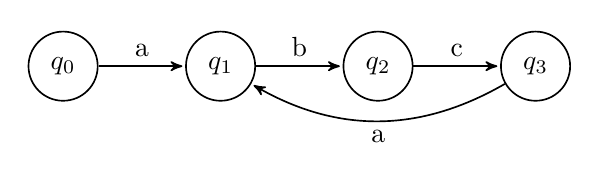
\begin{tikzpicture}[->,>=stealth',shorten >=1pt,auto,node distance=2cm,semithick]
	  \node[state] (A)              {$q_0$};
	  \node[state] (B) [right of=A] {$q_1$};
	  \node[state] (C) [right of=B] {$q_2$};
	  \node[state] (D) [right of=C] {$q_3$};          
	  \path
(A) edge  node {a} (B)
(B) edge  node {b} (C)
(C) edge  node {c} (D)
(D) edge [bend left]  node {a} (B)
;
	\end{tikzpicture}
  \end{center}
  \end{scriptsize}  
 \caption{\small Four-symbol four-state {\em regular automata} for recognizing the $\{(abc)^n : n \geq 1 \}$ language (\underline{$q_3$} is the acceptor state).}
\label{fig:regautomatae}
\end{figure}

In more detail, we randomly generated a $M=\{\mathcal{M}_1,\ldots,\mathcal{M}_{50}\}$ set of fifty different \strips\ models that encode different {\em regular automata}. Each $\mathcal{M}\in M$ encodes a different five-state {\em regular automata} with a five-symbol input alphabet. Each automata transition is encoded with a planning action. For instance, the execution of the {\em regular automatae} defined in Figure~\ref{fig:tautomatae}, with the sequence of input symbols $abcabc$, produces the following six-action plan {\small $(a,q_0\rightarrow q_1)$, $(b,q_1\rightarrow q_2)$, $(c,q_2\rightarrow q_3)$, $(a,q_3\rightarrow q_1)$, $(b,q_1\rightarrow q_2)$, $(c,q_2\rightarrow q_3)$}.

Here we assume that the actual applied transitions are unknown as well as the internal machine state. Assuming that the actual applied transitions is unknown means that the observation $\mathcal{O}(\pi,I)$ of the execution of a regular automata contains no actions, it is simply a sequence of states $\mathcal{O}(\pi,I)=\tup{s_1, \ldots , s_m}$. Assuming that the internal machine state is unknown means that $\mathcal{O}(\pi,I)$ is a $\Phi$-observation and that the $\Phi$ subset does not contain {\small\tt ($q$)} fluents, with $q\in Q$ and $q\neq q_0$. 

\subsubsection{Recognition of {\em Turing Machines}.} In this experiment the given models in $M$ represent different {\em Turing machines}~\cite{bylander1994computational,porco2013automatic}. Figure~\ref{fig:tautomatae} illustrate a seven-symbol six-state {\em Turing Machine} for recognizing the $\{a^nb^nc^n : n \geq 1 \}$ language. The {\em tape alphabet} is $\Sigma=\{a,b,c,x,y,z,\square\}$, the {\em input alphabet} $\Upsilon=\{a,b,c,\square\}$ and the machine states are $Q=\{q_0,q_1,q_2,q_3,q_4,\underline{q_5}\}$ (where \underline{$q_5$} is the only acceptor state).

Here we randomly generated a $M=\{\mathcal{M}_1,\ldots,\mathcal{M}_{50}\}$ set of fifty different \strips\ models that encode different five-symbol five-state {\em Turing Machines} with circular tapes. There is a planning action $a\in A$ for each machine transition, e.g. the full encoding of the {\em Turing Machine} of Figure~\ref{fig:tautomatae} produces a total of sixteen \strips\ action schema. With this regard, the execution of the {\em Turing Machine} defined in Figure~\ref{fig:tautomatae} with an initial tape $abc\square\square\square$ produces the eight-action plan {\small $(a,q_0\rightarrow x,r,q_1)$, $(b,q_1\rightarrow y,r,q_2)$, $(c,q_2\rightarrow z,l,q_3)$, $(y,q_3\rightarrow y,l,q_3)$, $(x,q_3\rightarrow x,r,q_0)$, $(y,q_0\rightarrow y,r,q_4)$, $(z,q_4\rightarrow z,r,q_4)$, $(\square,q_4\rightarrow \square,r,\underline{q_5})$}.

Again we assume that the actual applied transitions is unknown ($\mathcal{O}(\pi,I)$ contains no actions). Further, $\mathcal{O}(\pi,I)$ is a $\Phi$-observation and that the $\Phi$ subset does not contain {\small\tt $q$()} fluents, with $q\in Q$ and $q\neq q_0$ and that the values of several tape cells is unknown.

\begin{figure}
  \begin{scriptsize}
  \begin{center}
	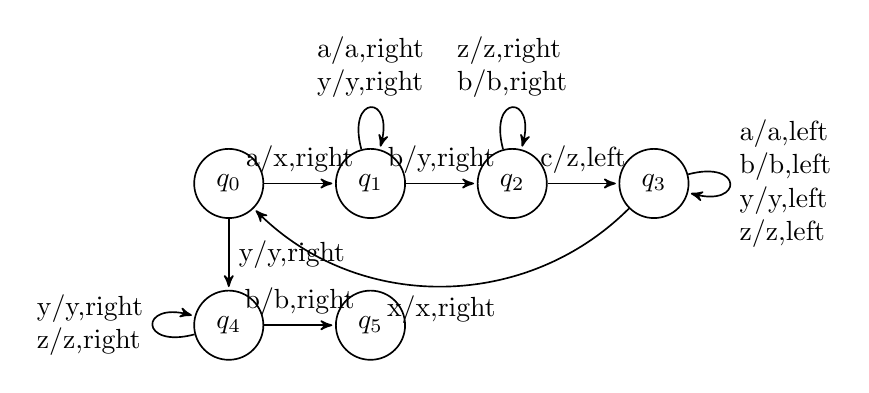
\begin{tikzpicture}[->,>=stealth',shorten >=1pt,auto,node distance=1.8cm,semithick]
	  \node[state] (A)              {$q_0$};
	  \node[state] (B) [right of=A] {$q_1$};
	  \node[state] (C) [right of=B] {$q_2$};
	  \node[state] (D) [right of=C] {$q_3$};
	  \node[state] (E) [below of=A] {$q_4$};
	  \node[state] (F) [right of=E] {$q_5$};                    

	  \path
(A) edge  node {a/x,right} (B)
(B) edge [align=left, loop above] node {a/a,right\\y/y,right} (B)
(B) edge  node {b/y,right} (C)
(C) edge [align=left, loop above] node {z/z,right\\b/b,right} (C)
(C) edge  node {c/z,left} (D)
(D) edge [align=left, loop right] node {a/a,left\\b/b,left\\y/y,left\\z/z,left} (D)
(D) edge [bend left=45] node {x/x,right} (A)

(A) edge  node {y/y,right} (E)
 (E) edge [align=left, loop left] node {y/y,right\\z/z,right} (E)
(E) edge  node {b/b,right} (F)
;
	\end{tikzpicture}
  \end{center}
  \end{scriptsize}  
 \caption{\small Seven-symbol six-state {\em Turing Machine} for recognizing the $\{a^nb^nc^n : n \geq 1 \}$ language.}
\label{fig:tautomatae}
\end{figure}


\subsubsection{Recognition of navigation models.} In this experiment the given models in $M$ represent different navigation models that are computed as the cross product of a regular automata with a four-operator \strips\ model for navigating a $n\times n$ grid.

In this case the regular automata constrain the applications of the navigation actions producing different navigation policies e.g. like the one in Figure~\ref{fig:model-example}. Given an observation of a plan execution, like the one illustrated at Figure~\ref{fig:grid-example}, here the task is to identify which navigation model produced that observation, despite the the applied actions are unobserved. In addition, for each observed state, only the value of fluents encoding the x and y coordinates of the agent are known while the value of the regular automata conditioning the navigation policy is unknown.


\subsection{Results}





\section{Conclusions}
\label{sec:conclussions}
This paper formalized the {\em model recognition} task and proposed, {\em model recognition as planning}, a method built on top of off-the-shelf classical planning algorithms to estimate the probability of a \strips\ model to produce a partial observation of a plan execution. The paper shows the effectiveness of {\em model recognition as planning} in a set of \strips\ models encoding different kinds of {\em automata}. {\em Model recognition as planning} succeeds to identify the executed automata despite the internal machine state or actual applied transitions, are unobserved.

In this work we do not assume that the observed agent is acting rationally, like in {\em plan recognition as planning}~\cite{ramirez2012plan,ramirez2009plan}. A related approach is recently followed for {\em model reconciliation}~\cite{Kambhampati:mreconciliation:ijcai17} where model edition is used to conform the PDDL models of two different agents. Also  related to this paper is the work on {\em Goal Recognition Design} but in that work the action model is given in advance and fixed~\cite{keren2014goal}.  


Previous work on the learning of \strips\ action models also defined semantic error metrics to quantify the errors of a model with respect to the observation of a plan execution~\cite{yang2007learning}. Our approach for quantifying this error is based on the definition of a edit distance for the model which allow us to not accumulate the repetition of errors coming from the the same model flaw.

Remarkably, the extension of this piece of work to the FOND planning setting~\cite{muise2012improved} is straightforward by simply considering the {\em all-outcomes} determiniztion of the actions with non-determinitic effects~\cite{yoon2007ff}. An interesting research direction is however to understand how to apply our approach to planning models where the planning models include actions with probabilistic effects~\cite{younes2005first}.  

\bibliographystyle{aaai}
\bibliography{planlearnbibliography}

\end{document}
